	\documentclass[10pt,twocolumn,letterpaper]{article}

\usepackage{cvpr}
\usepackage{times}
\usepackage{epsfig}
\usepackage{graphicx}
\usepackage{amsmath}
\usepackage{amssymb}
% Include other packages here, before hyperref.
\usepackage{hyperref}

\cvprfinalcopy % *** Uncomment this line for the final submission
\def\cvprPaperID{****} % *** Enter the CVPR Paper ID here
\def\httilde{\mbox{\tt\raisebox{-.5ex}{\symbol{126}}}}
% Pages are numbered in submission mode, and unnumbered in camera-ready
\ifcvprfinal\pagestyle{empty}\fi

% graphics pull from this folders
\graphicspath{{../figs/}}

\begin{document}
\title{Image Completion}

\author{Debora Sujono, Yue Tang \& Grace Yoo \\ 
University of Massachusetts Amherst \\ 
College of Information \& Computer Sciences \\
{\tt\small \{dsujono, gyoo, ytang\}@cs.umass.edu} \\
}

\maketitle

\section{Abstract} 
% no more than 300 words
We wanted to explore methods of completing images with missing pixel values. Networks that capture sequential information, such as a Recurrent Neural Network (RNN), are good candidates for image generation because they can be used to express a pixel value as a conditional probability. A modified version of a Convolutional Neural Network (CNN) was also used to assess the practicality of using a less complex model that is easier to compute. We found that our simplest model, a CNN with regression using mean squared error (MSE) loss, was extremely easy to run and the complex Pixel RNN didn’t produce images that were much more believable than the CNN with regression.

\section{Introduction}
% Introduction: this section introduces your problem, and the overall plan for approaching your problem
Image completion, also called content-aware fill or inpainting, is a generative technique that can be used to fill missing areas of an image. The desired result is an image that a human would perceive as normal. These techniques are often implemented in photo-editing software to mend corrupted images.

\par We can conceptualize a photograph as a low-dimensional sample from a high-dimensional distribution, the original scene. The problem can be framed as learning these high-dimensional distributions such that we can generate a sample that approximates missing pixels. In our project, an incomplete image is treated as the lower-dimensional sample from the complete image. Contextual information from incomplete images, such as the values of pixels neighboring the missing content, can help inform the generative model. \\

%TODO n layer model
\par 
We will experiment with training generative models on observations of incomplete images $X$, and targets of original images $y$. The original images are from the CIFAR-10 dataset, and the incomplete versions have a square region removed from the center of the image. Using Recurrent Neural Networks (RNNs) and Convolutional Neural Networks (CNNs), we will attempt to learn neuron weights to attempt modeling the area in $y$ corresponding to the missing region. We will randomly generate samples from these predictions, insert them into incomplete images, and use human judgment to determine if the predicted images are plausible. As a technical means of evaluation, we will use root mean squared error (RMSE) between $\hat y$ and $y$ to measure how different the images are. However, our main goal is to be able to complete images in general, which is why our hold out test set is comprised of incomplete images unknown to the model. For this reason, we don't consider RMSE to be the most important metric.\\

Our simplest model is a n layer CNN with regression between $X$ and $y$, using RMSE loss. We also used RNNs designed to read pixels sequentially; one model used a pre-existing implementation of pixel RNN with sigmoidal output, the other model had 256-way categorical cross-entropy ("softmax loss"). We also used an adaptation of CNNs designed to emulate the sequential information feeding within a recurrent layer. We expected that the complex models, which sequentially approximate the joint distribution for each pixel, would outperform the simpler CNN using regression.\\

\section{Related Work} 
% This section discusses relevant literature for your project
Training a generative model can easily become intractable; we not only have to simulate high dimensional distributions, but also apply some kind of inference method to create a new sample. We decided to stick with feed-forward networks, where at test time the input is the incomplete image, and the output is the completed image. The following sections detail previous implementations of RNNs and CNNs adapted for sequentially scanning pixels in images.

\subsection{Pixel Recurrent Neural Networks}
The recurrent layers of an RNN have memory-like properties, which is why networks using specialized types of recurrent layers are called Long-Short Term Memory (LSTM) nets. These variants on recurrent layers were designed to ameliorate the exploding gradient sometimes experienced by vanilla recurrent layers. We think that the reason this happens in vanilla layers because feed forward networks with great depth generally have the potential for exploding gradients. At a high level, the way in which recurrent layers store previous information needs to be adjusted, in order to remember larger global patterns over iterations. LSTMs have a feature in recurrent layers, sometimes called a "gate", which determines if information from the previous cell will be fed forward, or forgotten. This gate is the hidden layer activation function, which for vanilla RNNs is often a sigmoid function. \cite{handwritingRNN}\\

% handwriting RNN paper
RNNs were used to generate convincing script from samples of handwriting. Previously, the handwriting generation problem posed a challenge because while the contextual information to generate individual letters may have been available from some models, many failed to learn higher-level sequences, such as stringing letters together. \cite{handwritingRNN} This seems particularly important in creating convincing samples of cursive handwriting styles. The cursive handwriting results from the network described by the Graves paper are pretty convincing. The inpainting problem is similar to handwriting generation in that it is important to preserve sequential features within and across layers.\\

% main pixel RNN paper
A study aimed to improve the efficiency of RNN architectures experimented with two different implementations of LSTMs that differed in the way they scanned across an image, collecting sequential data. The Row LSTM scans an image row by row, from top to bottom. The Diagonal Bidirectional LSTM (BiLSTM) simultaneously scans an image from the top left to the bottom right corner and from the top right to the bottom left corner. By skewing the inputs in a particular way, both diagonals are computed efficiently. The first step of the scanning is accomplished by a $1 \times 1$ convolution filter, which creates a tensor of $4h \times n \times n$ for $h$ hidden states and image with size $n \times n$. This can be thought of as a sliding mask. The second step is a column-wise sweep with a $2  \times  1$ convolution filter, which isn't masked. This is the part that facilitates recurrence within the layer. The authors noted that because the Diagonal LSTM already has a good receptive field with the second $2  \times  1$ kernel, increasing the size shouldn't improve the receptive field much. For both types of Pixel RNNs, van den Oord et al. suggest that networks can have up to 12 layers. A downside of LSTM layers is that you cannot parallelize the processes, as they must be computed sequentially \cite{pixelRNN}. \\

\subsection{Pixel Convolutional Neural Networks}
CNNs, despite lacking some kind of inherent sequential structure, can be modified to emulate the scanning accomplished by LSTM layers, without the cost associated with sequential computations. Using a convolutional filter to capture smaller areas of images and compute features within those receptive fields is a way to create a sliding mask over an image \cite{pixelRNN}. These computations can be parallelized, which makes the Pixel CNN worth exploring, since we weren't certain how long Pixel RNN would take to train. \\

\section{Approach}
% Approach: This section details the framework of your project. Be specific, which means you might want to include equations, figures, plots, etc
The networks we're using are all different types of feed forward networks. These feed forward networks have the same input and output. The input training data $X$ for the networks are all comprised of incomplete $32 \times 32 \times 3$ CIFAR-10 images. The training labels $y$ are the complete, original CIFAR-10 images. In the following sections, we will outline the different training methods that we will run. Once we train networks that we can generate samples from, we'll use them to create filled-in images $\hat{y}$. The Pixel RNN and Pixel CNN implementations are built on a forked github repository called 'pixel\_rnn' \cite{igul_github}. \\

\subsection{Networks}
To compare the networks performances, we will use Root Mean Squared Error (RMSE) between predicted samples $\hat y$ and original targets $y$. The RMSE will give us an idea of how well our generated images compare to the originals; however, the problem is to generate any plausible images, so we will also randomly sample images for human judgment. We will ask judges to rate an image as "plausible" or "not plausible", and determine which models generate the most believable images. If a sufficient number of samples are generated, we will calculate inter-annotator agreement for the samples across human judges. \\

\subsubsection{CNN with Regression}
\par We implemented a CNN with mean squared error (MSE) loss between incomplete and original images, to perform regression on the intensities of the missing pixels. Note that while we're using regression, because of the Rectified Linear Units (ReLUs), this is still  a nonlinear network. \\

%%%%%%%%%%%%%%% CNN regression ARCHITECTURE
We have implemented a 3-layer CNN with regression using the following architecture: 
\begin{itemize}
\item Input: $32  \times  32  \times  3$ raw pixel values
\item 2 of these layers:
\subitem Convolutional layer with $7  \times  7$ filter
\subitem ReLU activation
\subitem Max Pooling layer $2  \times  2$
\item Fully-Connected Layer
\item ReLU activation with MSE loss
\end{itemize}
\

\subsubsection{Pixel RNN}
Pixel RNNs approximate the joint distribution of pixels in the image by treating each pixel as a product of conditional distributions of all pixels previously seen in that layer.  This converts the problem into a sequence problem, and the task becomes to predict the next pixel given the previously generated ones \cite{pixelRNN}. 

Let $p(x)$ be the generated distribution for image $x$ with dimensions $n \times n$, represented as a row of length $n^2$. We approximate $p(x_i)$ by: \\
\
$p(x) = \prod_{i=1}^{n^2} p(x_i | x_1, ... , x_{i-1} )$ \\

For a 3-channel RGB image, the red channel pixels should be fed first, followed by green, and finally blue. The approximation of color pixel $p(x_i | x_{<i})$ is then: \\
\
$p(x_i | x_{<i}) = p(x_{i,R} | x_{<i}) * p(x_{i,G} | x_{<i}, x_{i,R}) * p(x_{i,B} | x_{<i}, x_{i,R}, x_{i,G}) $ \\

This formula illustrates how the blue channel is dependent on the green and red channels, and the green channel is dependend on the red channel, and the red channel is independent of the other channels. The version of Pixel RNN we adapted was using a sigmoid layer for the final output. We thought that the 256-way "Softmax loss" (categorical cross-entropy) would be a better way to output a sample, so we implemented that as it was described in the paper "Pixel Recurrent Neural Networks" \cite{pixelRNN}. \\

We have implemented a 12-layer Pixel RNN with the following architecture: 
%%%%%%%%%%%%%%% pixel RNN ARCHITECTURE
\begin{itemize}
\item Input: $32  \times  32  \times  3$ raw pixel values
\item $7 \times 7$ convolution (mask)
\item 2 of these layers:
\subitem Diagonal LSTM
\subsubitem $1 \times 1$ convolution (mask)
\subsubitem $2 \times 1$ convolution (no mask)
\item 2 of these layers:
\subitem $1  \times  1$ convolution (mask)
\subitem ReLU
\item Output: 256-way Softmax loss
\end{itemize}
\

\subsubsection{Pixel CNN}
Following the guidelines from the paper "Pixel Recurrent Neural Networks" \cite{pixelRNN}, We have implemented a 15-layer Pixel RNN with the following architecture: 
%%%%%%%%%%%%%%% pixel CNN ARCHITECTURE
\begin{itemize}
\item Input: $32  \times  32  \times  3$ raw pixel values
\item $7 \times 7$ convolution (mask)
\item 4 of these layers:
\subitem $3 \times 3$ convolution (mask)
\subitem ReLU
\item 2 of these layers:
\subitem $1 \times 1$ convolution (mask)
\subitem ReLU
\item Output: Sigmoid activation
\end{itemize}
\

\section{Experiments} 
% This section begins with what kind of experiments you're doing, what kind of dataset(s) you're using, and what is the way you measure or evaluate your results. It then shows in details the results of your experiments. By details, we mean both quantitative evaluations (show numbers, figures, tables, etc) as well as qualitative results (show images, example results, etc).
\subsection{Data}
We used the CIFAR-10 dataset, which consists of $60,000$ images evenly distributed into 10 classes (airplane, automobile, bird, cat, deer, dog, frog, horse, ship, truck). Each $32 \times 32 \times 3$ pixel image is represented by the RGB color model, so it has 3 channels. We will remove a $16 \times 16$ region of each image, and consider the original image to be the original distribution of $32 \times 32 \times 3 = 3,072$ dimensions. All images have normalized pixel intensities. \\

This is what our incomplete images look like after we remove the center pixels.\\
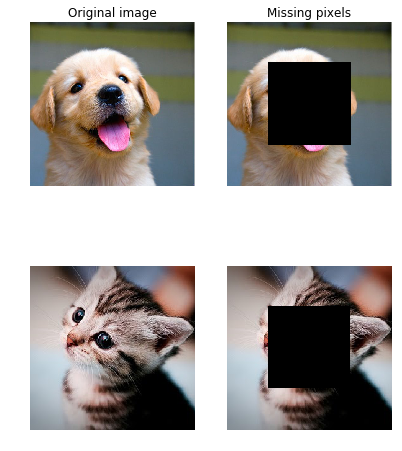
\includegraphics[width=1.0\linewidth]{img_sample.png}

%% how much in train and test set
We used 50,000 images for training and 10,000 images for testing. The testing images were not seen during training.

\subsection{Setup}
In order to run the models, we had to use the Elastic Cloud product offered by Amazon Web Services. We used the Amazon Marketplace Image (AMI) called \textit{cs231n \_caffe \_torch7 \_keras \_lasagne \_v2}, developed by the CS231N course \cite{aws_tutorial}. We set it up on a g2.xlarge instance, which was limited to spot requests. 

\subsection{Results}
Table 1 shows the RMSE values for the models, as well as the number of samples deemed to be convincing by human judges. If the entry in the table is not filled, it means that our model never finished training to the point where we could generate samples.
\begin{table}[!ht]
\centering
\caption{Each of 3 human judges saw 10 samples each, totaling 30 total samples for each model}
\begin{tabular}{lll}
\hline
Model               & Test RMSE & \# Convincing samples \\ \hline
CNN with Regression & 24.468    &  4                     \\
Pixel RNN w Sigmoid &   -       &  -                     \\
Pixel RNN w Softmax &           &  10                     \\
Pixel CNN           &   -       &  -                     \\ \hline
\end{tabular}
\end{table}

\subsection{Generated Samples}
\textbf{CNN with Regression}
Samples from training: the images in the top row are the original and the incomplete, respectively. \\
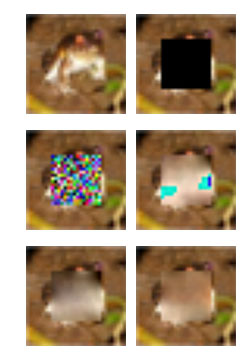
\includegraphics[width=0.8\linewidth]{baseline_train_frog.jpg} 
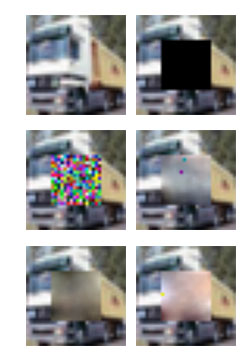
\includegraphics[width=0.8\linewidth]{baseline_train_truck.jpg} 

Samples from testing: the left column is the original image, the right column is the inpainted image \\
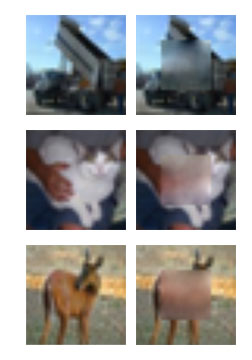
\includegraphics[width=0.8\linewidth]{baseline_test.jpg} 

\textbf{Pixel RNN w Softmax}
Samples from training: the images in the top row are the original and the incomplete, respectively. \\
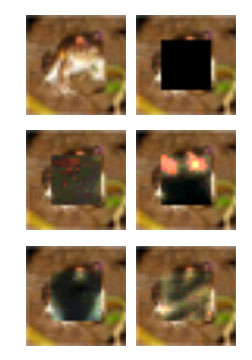
\includegraphics[width=0.8\linewidth]{rnn_rgb_train_frog.jpg} 
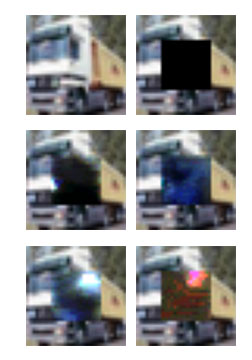
\includegraphics[width=0.8\linewidth]{rnn_rgb_train_truck.jpg} 

Samples from testing: the left column is the original image, the right column is the inpainted image \\
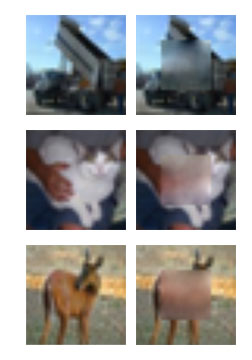
\includegraphics[width=0.8\linewidth]{baseline_test.jpg} 

\section{Conclusion}
% Conclusion: What have you learned? Suggest future ideas.
Our results, although we don't have many of them, suggest that Pixel RNN is better for image completion than Pixel CNN. We expected this to be the case. One thing we didn't expect was to find that the Pixel RNN didn't perform that much better than the CNN with regression. The Pixel RNN, although it was made faster by the Diagonal BiLSTM layers, was still very slow. Training with 8 gpus on a g2.xlarge instance took days. The multi-scale version of Pixel RNN described by van der Oord et al. describes an implementation that takes advantage of the parallelized computations allowed by Pixel CNN, by combining unconditional as well as conditional generative networks \cite{pixelRNN}. \\

A big aspect of the learning done in this project is the practical experience of standing up a model on GPU computing. One particularly important lesson we learned is that because training outcomes for these models can be sensitive to the number of training examples, iterations, or epochs, models that can be fully run in a short amount of time are more likely to be well-tuned. Being inexperienced with using the AWS cluster services, we underestimated the limitations of access to p2 or g2 instances. We weren't able to tune hyperparameters for the Pixel RNN models on the full datasets, since they took so long to train. Within the scope of our project and our results, we find that images we were able to generate with the complex Pixel RNN, which took days to train, weren't that much more convincing than the ones generated by the simpler CNN with Regression.\\

We received a helpful suggestion that using photos from the same domain would improve the performance of our models. By running the same models on a face dataset, we might have achieved better results, such as those achieved by van der Oord et al. with a variant of the Pixel CNN \cite{pixelCNN}. Another idea to consider is ordering the training examples for the RNNs such that we feed all the airplane pictures in a chunk, so that airplane specific features can be persisted across layers, rather than feeding a randomized assortment of images from different classes.\\

Improving our evaluation system would be a worthwhile next step. If we improve the way we collect annotations from human judges such that we have a large volume of them, we could calculate statistics such as inter-annotator agreement and determine if certain images are harder to complete in a convincing way. We could also replace the RMSE as a method of technically comparing model performances, since it doesn't accurately capture our goal. Contextual loss, which measures the context similarity between the generated region of an image with the rest of the image, is one possible loss function. Perceptual loss is meant to encourage a network to create samples that are similar to those already seen in training. These losses are described in a paper that uses Generative Adversarial Networks (GANs) to solve image completion \cite{inpaint}. An implementation of contextual and perceptual loss for Pixel RNN and Pixel CNN would be a great addition to this project. \\

\begin{thebibliography}{1}
\bibitem{pixelRNN} Pixel Recurrent Neural Networks \url{https://arxiv.org/pdf/1601.06759v3}
\bibitem{handwritingRNN} Generating Sequences with Recurrent Neural Networks \url{https://arxiv.org/pdf/1308.0850v5.pdf}
\bibitem{pixelCNN} Conditional Image Generation with PixelCNN Decoders \url{https://arxiv.org/pdf/1606.05328v2.pdf}


\bibitem{igul_github} \url{https://github.com/igul222/pixel_rnn}
\bibitem{aws_tutorial} \url{http://cs231n.github.io/aws-tutorial/}

\bibitem{inpaint} Semantic Image Inpainting with Perceptual and Contextual Losses \url{https://arxiv.org/pdf/1607.07539v2.pdf}
\end{thebibliography}


\end{document}
